\begin{figure}
  \centering
  \sffamily % font family for labels (does not include legend)
  % subfigure A
  \begin{tikzpicture}
    \node[anchor=north west] at (-1em, 0em) {% label
      \textbf{A}
    };
    \node[anchor=north west] at (0em, 0em) {% image
      \begin{subcaptionblock}{0.25\textwidth}
        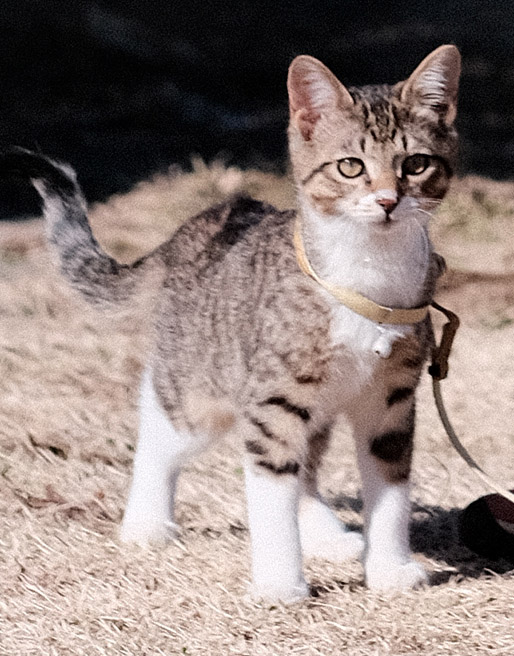
\includegraphics[width=\textwidth]{one_cat.jpg}
        \phantomcaption\label{cat}
      \end{subcaptionblock}
    };
    \node[% inner label
      anchor=north west,
      fill=white,
      fill opacity=0.8,
      text opacity=1,
      inner sep=0.2em
    ] at (1ex, -1ex) {WT};
  \end{tikzpicture}
  \hfill
  % subfigure B
  \begin{tikzpicture}
    \node[anchor=north west] at (-1em, 0em) {
      \textbf{B}
    };
    \node[anchor=north west] at (0em, 0em) {
      \begin{subcaptionblock}{0.62\textwidth}
        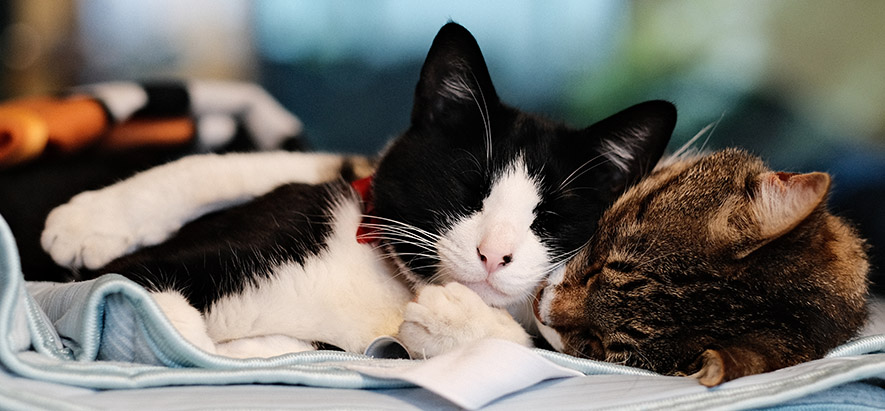
\includegraphics[width=\textwidth]{two_cats.jpg}
        \phantomcaption\label{twocats}
      \end{subcaptionblock}
    };
  \end{tikzpicture}
  % main caption
  \caption{Some cats.
   In \subref{cat}, a single cat being cute.
   \subref{twocats} shows increased cuteness associated with a higher number of cats.}
  \label{fig:cats}
\end{figure}